\chapter{Objetivos}
\label{cap:capitulo2}


En esta sección se describirá el problema a resolver junto con los objetivos y requisitos pautados en el desarrollo del TFG


\section{Descripción del problema}
\label{sec:descripcion}

Como anteriormente hemos relatado, los drones tienen un uso actualmente elevado para solventar tareas de alta complejidad adoptado de sensores 
para ello. El objetivo principal de este TFG, es desarrollar un comportamiento de navegación autónoma basado en aprendizaje por refuerzo e 
inteligencia artificial, en el que el dron sea capaz de desenvolverse por escenarios urbanos. El enfoque de este trabajo de investigación 
se centrará en la creación de una solución eficiente y completa ante la problemática que puede llegar a tener la navegación autónoma, se 
mostrará un comportamiento capaz de realizar el seguimiento de un carril para demostrar la complejidad de mantener una trayectoria estable 
y precisa utilizando en un vehículo autónomo aéreo. 

A continuación, se definen los siguientes subobjetivos: 

\begin{enumerate}
    \item Análisis y desarrollo de un sistema perceptivo basado en redes neuronales en la navegación autonónoma de drones.
    \item Desarrollo  de un sistema de control para drones utilizando técnicas de Reinforcement Learning para lograr una navegación 
    autónoma y segura.
    \item Analisis y desarrollo de una aplicación de navegación autónoma de drones basandonos en el seguimiento de un carril.
    \item Análisis y comparativas de los diferentes comportamientos desarrollados en este trabajo con el fin de 
    lograr resultados interesantes acerca de la utilización de redes neuronales y aprendizaje por refuerzo en la navegación autónoma de drones.
    \item Desarrollo en ROS para intercomunicar componentes en la navegación autonónoma del dron.
\end{enumerate}
\newpage
\section{Requisitos}
\label{sec:requisitos}

Los requisitos que han de cumplirse en este trabajo son: 
\begin{enumerate}
    \item Uso del vehículo UAV en el entorno de simulación fotorrealista Airsim junto a UnRealEngine.
    \item El comportamiento robusto y en tiempo real para garantizar la navegación segura del vehículo.
    \item Los sistemas desarrollados deben ser reactivos para poder reaccionar a su entorno de manera concisa y eficiente.
    \item Comportamiento portable sin reconfiguración.
\end{enumerate}


\section{Metodología}
\label{sec:metodologia}

Este trabajo, comenzó oficialmente en Septiembre del 2023 aunque en Diciembre del 2022 se plantearon varias ideas a desarrollar, y se finalizó en Mayo del 2024. \\

La metodología que se llevo a cabo fue:

\begin{enumerate}
    \item Reuniones semanales mediante Teams\footnote{\url{https://www.microsoft.com/es-es/microsoft-teams/group-chat-software}} con una duración de media o una hora, con el fin de tener un control semanal y pactar los objetivos semanales a seguir. Gracias a estas reuniones, se tenia una organización global del proyecto. 
    \item Contacto via email de la universidad con el fin de solventar problemas urgentes. 
    \item Utilización de la metodología Espiral\footnote{\url{https://www.lifeder.com/modelo-espiral/}}: Este tipo de metología consiste en llevar a cabo
    un cicle iterativo que se debe repetir hasta que se alcanze el objetivo y se componen de varias fases:
    \begin{itemize}
      \item \textbf{Fase 1: Definir los objetivos y descripciones de las condiciones generales}. Consiste en marcar los objétivos que se deben seguir a la misma vez de barajar posibles 
      alternativas especificando las condiciones (por ejemplo, sistema operativo, entornos, lenguajes de programación, herramientas de desarrollo). En esta fase nosotros definimos el tipo
      de aplicación que se iba a seguir que es la navegación autónoma de drones considerando un entorno de simulación de carreteras. También de identificar alternativas técnologias como utilizaremos
      Airsim para una simulación fotorrealista, integrar el middleware ROS para la comunicación y control, emplear PX4 Autopilot,Mavros u otras herramientas para el control de vuelo. \newline
      \item \textbf{Fase 2: Análisis de requisitos}. Se realiza una investigación y documentación sobre las restricciones que podemos llegar a tener, entornos de trabajo, objetivos. Realizamos
      un análisis sobre el uso que conllevaba utilizar el simulador Airsim junto con el midllware robótico ROS, qué tipo de compatbilidad puede llegar a tener, fiabilidad en cuanto 
      a la comunicación entre ellos, viabilidad con herramientas como PX4 Autopilot con Airsim. \newline

      \item \textbf{Fase 3: Desarrollo y pruebas}. Se realiza la construcción de la arquitectura del sistema como de sus componentes y comunicación entre ellos para llevar acabo la aplicación 
      marcada como objetivo en la fase 1 como la configuración del entorno en Airsim, configuración del modelo del dron, integración con ROS y configuraciones de bibliotecas. Conllevando
      al desarrollo de los algoritmos y realización de diferentes pruebas.\newline

      \item \textbf{Fase 4: Evaluación}. Se trata de presentar el sistema desarrollado recompilando problemas, mejoras a seguir, pruebas de diferentes algoritmos y sus resultados. Recopilaremos
      diferentes pruebas realizadas, su uso, rendimiento, optimizaciones, gráficas con diferentes comparativas de diferentes comportamientos en cuanto a control.  \newline

      \item \textbf{Planificación del próximo ciclo}. Al ser un método en espiral, cuando se completa un ciclo se comienza la planificación del siguiente ciclo. Dicha planificación 
      sigue normalmente si se alcanzó el objetivo del anterior ciclo, planteandose los objetivos del siguiente ciclo. También podría ser encontrar nuevas soluciones si en alguna de las 
      otras etapas se ha producido problemas, hasta de poder cambiar estrategias existentes por nuevas alternativas previamente definidas. En este trabajo hemos realizo varios ciclos compuestos
      por la definición del problema, los ánalisis del entorno de simulación e infraestructuras y construcción del sistema perceptivo-control del robot, además de marcar nuevos 
      objetivos dados por los problemas que nos hemos llegado encontrando en este desarrollo. 

    \end{itemize}
  
    A lo largo del desarrollo de este TFG, se marcaron estas 4 fases estando en un ciclo iterativo junto con los objetivos a seguir permitiendo cambios y mejoras continuas hasta llegar al resultado final.

    \begin{figure} [H]
        \begin{center}
          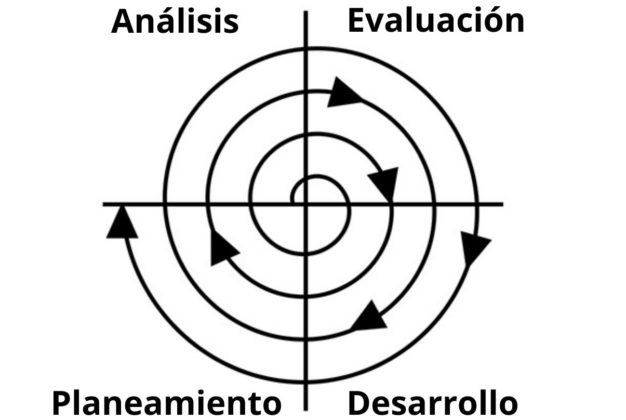
\includegraphics[scale=0.5]{figs/objetivos/espiral.jpg}
        \end{center}
        \caption{Ilustración de metología en Espiral }
        \label{fig:Espiral}
      \end{figure}
  
    \item Tener un control de versiones mediante la plataforma GitHub\footnote{\url{https://github.com/RoboticsLabURJC/2022-tfg-barbara-villalba}}, con el objetivo de tener un almacenamiento de código y respaldos de ello.  
    \item El uso de un blog \footnote{\url{https://roboticslaburjc.github.io/2022-tfg-barbara-villalba/}}, en el cual se describió brevemente los pasos que se siguieron para el desarrollo del TFG.
\end{enumerate}

\begin{figure} [H]
    \begin{center}
      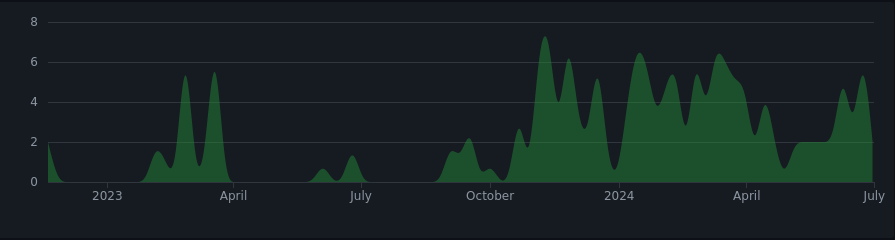
\includegraphics[width=0.9\textwidth,height=0.3\textwidth]{figs/objetivos/github.png}
    \end{center}
    \caption{Seguimiento de trabajo en GitHub}
    \label{fig:github}
  \end{figure}


\section{Plan de trabajo}
\label{sec:plantrabajo}

Finalmente, los pasos a seguir de este trabajo han sido: 
\begin{enumerate}
    \item Comienzo del trabajo. 
    \begin{itemize}
        \item Búsqueda del problema a desarrollar y análisis del estado del arte del uso de los drones en aplicaciones robóticas.
        \item Instalación de las diferentes librerías y aplicaciones de software. 
        \item Preparación de configuración de toda la infraestructura, teniendo un análisis y estudio de comunicaciones para poder comenzar con el desarrollo. 
    \end{itemize}
    \item Desarrollo: Una vez se tuvo listo toda la infraestructura tanto de comunicaciones como de librerías de software, se dio a pie el comienzo del desarrollo del código
        \begin{itemize}
            \item En primer lugar, se desarrollo un teleoperador sencillo del drone para ver el funcionamiento del vehículo y dicho comportamiento.
            \item Una vez finalizada la tarea del teleoperador, se comenzó con los algoritmos de percepción de detencción de carril mediante redes neuronales.
            \item Análisis y comparación de los resultados de los diferentes modelos que ofrece la red neuronal escogida con el propósito de tener la mejor solución. 
            \item El siguiente paso fue estudiar la posibilidad de tener un algoritmo de aprendizaje no supervisado llamado clustering para clasificar las diferentes lineas que aparezcan en el escenario de la carretera.
            \item Desarrollo del algoritmo de percepción junto con los dos puntos anteriormente mencionados.
            \item Con el fin del algoritmo de percepción, se comenzó el desarrollo de un controlador sencillo PID para ver el funcionamiento de la percepción y de la navegación en el vehículo. 
            \item A continuación, fue la programación del algoritmo de aprendizaje por refuerzo para el seguimiento del carril.
        \end{itemize}
    \item Evaluación: Se realizo la comparativa de los resultados obtenidos en el aprendizaje por refuerzo.
        
    \item Redacción de la memoria del trabajo para la documentación de todo el proceso de investigación realizado. 
\end{enumerate}


